\section{Posets of graph rewriting events}

\subsection{From transition systems to posets of events}

\begin{lemma}
\label{lemma:pos_infl}
Let $TS = (Q,R,E,T,I,<,\dashv)$ be a transition system and let $e_1,e_2 \in E$.
$e_1< e_2\implies \labl(e)\xrightarrow{+}\labl(e')$.
\end{lemma}
\begin{proof}
  From~\autoref{def:seq_dep} $e_1 < e_2$ implies there exists two transitions $M\overset{m_1,p_1}{\Rightarrow} M_1$ and $M_1\overset{m_2,p_2}{\Rightarrow} M_2$ that are sequential dependent. For any such pair of transitions, using~\autoref{lem:completeness_causal_pair} there exists a causal pair which in turns implies that $\labl(e)\xrightarrow{+}\labl(e')$.
\end{proof}

\begin{definition}[Story]
  Let $TS = (Q,R,E,T,I,<,\dashv)$ be a transition system.
  A \emph{story} $s = (E_s,<_s,\dashv_s)$ is a subset of events $E_s\subseteq E$ equipped with two binary relations on events $<_s$, $\dashv_s$ which are the restrictions of $<$ and $\dashv$ respectively, to the set $E_s$.
\end{definition}

Instead of working on the transition system, we interpret ou logic over a set of stories, $\mathcal{S}$ with the constraint that $\mathcal{S}$ is closed under set inclusion: $s\in \mathcal{S} \implies \forall s'\subset_{\labl} s, s'\in\mathcal{S}$.
%We are not interested in the extraction mechanism, as long as the identity of events and the relationships between them (causality and inihibition) are preserved.

\bigskip

In interpreting our logic, we only work with the posets in $\mathcal{S}$ without having access to the transition system. If we are interested in the relations between events inside a poset, for example $e_1<_s e_2$, those are available in the structure of the poset. However, if we want to interpret formulas that relate events in different posets, we need to retrieve these relations from the events \emph{itselves}.

%Thus we need to fix some structure into the events, and we will do that by considering the category of simple graphs and transition system based on graph rewriting.

\subsection{Refinement of graph rewriting rules}

Let $r_1$ and $r_2$ two rules such that there exists a positive influence between the two : there exists $O$ such that $r_1 \redl{+}_O r_2$. Let us define a refinement of the two rules
such that the following diagram commutes:
\[
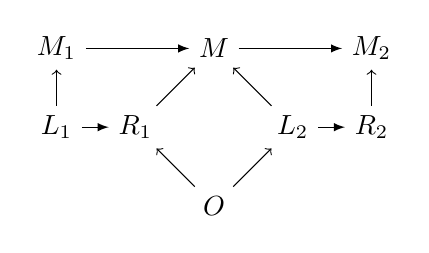
\begin{tikzpicture} %[scale=0.8]
  \node (o) at (0,-1) {\(O\)};
  \node (p) at (0,1) {\(M\)};
  \node (r1) at (-1,0) {\(R_1\)};
  \node (l1) at (-2,0) {\(L_1\)};
  \node (l2) at (1,0) {\(L_2\)};
  \node (r2) at (2,0) {\(R_2\)};
  \node (m1) at (-2,1) {\(M_1\)};
  \node (m2) at (2,1) {\(M_2\)};
  \draw [->] (l1) -- (m1);
  \draw [->] (r2) -- (m2);
  \draw [->] (o) -- (r1);
  \draw [->] (o) -- (l2);
  \draw [->] (r1) -- (p);
  \draw [->] (l2) -- (p);
  \draw [>=latex, ->] (m1) -- (p);
  \draw [>=latex, ->] (p) -- (m2);
  \draw [>=latex, ->] (l1) -- (r1);
  \draw [>=latex, ->] (l2) -- (r2);
\end{tikzpicture}
\]
We compute $M$ as the pushout of the span $R_1\remb O\lemb L_2$ and using the Dpo graph rewriting we compute the two $M_1$ and $M_2$. We can then refine the two rules to the sequence $M_1\action M\action M_2$. We call $M$ the context which realises the positive influence between $r_1$ and $r_2$.

In a poset, we have that for any event, its immediate causes have a positive influence on it (\autoref{prop:cause_pos_infl}). Hence we can refine events in a poset and propagate the context.

\begin{example}
\label{ex:e1e2e3}
Let us consider the poset $e_1<e_2<e_3$ with $\labl(e_1)=r_1$, $\labl(e_2)=r_2$ and $\labl(e_3)=r_3$. First we compute the two contexts for $r_1\redl{+}_{O_1} r_2$ and $r_2\redl{+}_{O_2} r_3$:
\[
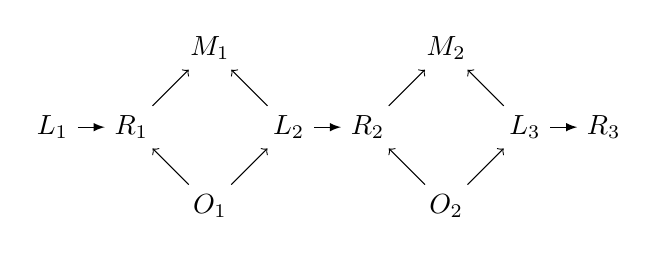
\begin{tikzpicture} %[scale=0.8]
  \node (o1) at (0,-1) {\(O_1\)};
  \node (m1) at (0,1) {\(M_1\)};
  \node (r1) at (-1,0) {\(R_1\)};
  \node (l1) at (-2,0) {\(L_1\)};
  \node (l2) at (1,0) {\(L_2\)};
  \node (r2) at (2,0) {\(R_2\)};
  \node (o2) at (3,-1) {\(O_2\)};
  \node (m2) at (3,1) {\(M_2\)};
  \node (l3) at (4,0) {\(L_3\)};
  \node (r3) at (5,0) {\(R_3\)};
  \draw [->] (o1) -- (r1);
  \draw [->] (o1) -- (l2);
  \draw [->] (r1) -- (m1);
  \draw [->] (l2) -- (m1);
  \draw [->] (o2) -- (r2);
  \draw [->] (o2) -- (l3);
  \draw [->] (r2) -- (m2);
  \draw [->] (l3) -- (m2);
  \draw [>=latex, ->] (l1) -- (r1);
  \draw [>=latex, ->] (l2) -- (r2);
  \draw [>=latex, ->] (l3) -- (r3);
\end{tikzpicture}
\]
We then apply the rewriting of $M_1$ using $r_2$ and combine the context with $M_2$:
\[
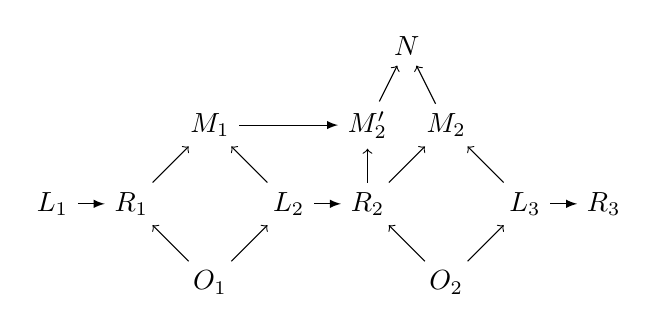
\begin{tikzpicture} %[scale=0.8]
  \node (o1) at (0,-1) {\(O_1\)};
  \node (m1) at (0,1) {\(M_1\)};
  \node (r1) at (-1,0) {\(R_1\)};
  \node (l1) at (-2,0) {\(L_1\)};
  \node (l2) at (1,0) {\(L_2\)};
  \node (r2) at (2,0) {\(R_2\)};
  \node (o2) at (3,-1) {\(O_2\)};
  \node (m2) at (3,1) {\(M_2\)};
  \node (l3) at (4,0) {\(L_3\)};
  \node (r3) at (5,0) {\(R_3\)};
  \node (m2p) at (2,1) {\(M_2'\)};
  \node (n) at (2.5,2) {\(N\)};
  \draw [->] (o1) -- (r1);
  \draw [->] (o1) -- (l2);
  \draw [->] (r1) -- (m1);
  \draw [->] (l2) -- (m1);
  \draw [->] (o2) -- (r2);
  \draw [->] (o2) -- (l3);
  \draw [->] (r2) -- (m2);
  \draw [->] (l3) -- (m2);
  \draw [->] (m2) -- (n);
  \draw [->] (m2p) -- (n);
  \draw [->] (r2) -- (m2p);
  \draw [>=latex, ->] (l1) -- (r1);
  \draw [>=latex, ->] (l2) -- (r2);
  \draw [>=latex, ->] (l3) -- (r3);
  \draw [>=latex, ->] (m1) -- (m2p);
\end{tikzpicture}
\]
Finally, we apply the rewriting steps on $N$ and obtain the refined sequence : $N_0\action N_1\action N\action N_3$:
\[
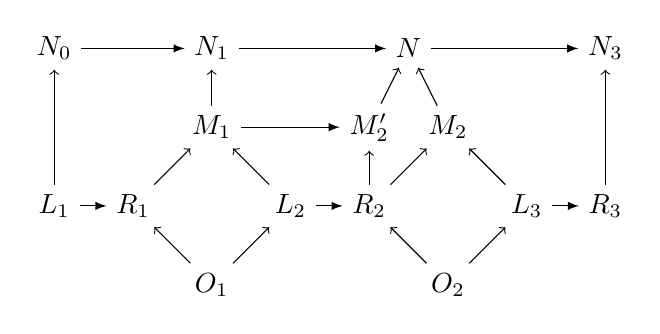
\begin{tikzpicture} %[scale=0.8]
  \node (o1) at (0,-1) {\(O_1\)};
  \node (m1) at (0,1) {\(M_1\)};
  \node (r1) at (-1,0) {\(R_1\)};
  \node (l1) at (-2,0) {\(L_1\)};
  \node (l2) at (1,0) {\(L_2\)};
  \node (r2) at (2,0) {\(R_2\)};
  \node (o2) at (3,-1) {\(O_2\)};
  \node (m2) at (3,1) {\(M_2\)};
  \node (l3) at (4,0) {\(L_3\)};
  \node (r3) at (5,0) {\(R_3\)};
  \node (m2p) at (2,1) {\(M_2'\)};
  \node (n) at (2.5,2) {\(N\)};
  \node (n0) at (-2,2) {\(N_0\)};
  \node (n1) at (0,2) {\(N_1\)};
  \node (n3) at (5,2) {\(N_3\)};
  \draw [->] (o1) -- (r1);
  \draw [->] (o1) -- (l2);
  \draw [->] (r1) -- (m1);
  \draw [->] (l2) -- (m1);
  \draw [->] (o2) -- (r2);
  \draw [->] (o2) -- (l3);
  \draw [->] (r2) -- (m2);
  \draw [->] (l3) -- (m2);
  \draw [->] (m2) -- (n);
  \draw [->] (m2p) -- (n);
  \draw [->] (r2) -- (m2p);
  \draw [->] (l1) -- (n0);
  \draw [->] (m1) -- (n1);
  \draw [->] (r3) -- (n3);
  \draw [>=latex, ->] (l1) -- (r1);
  \draw [>=latex, ->] (l2) -- (r2);
  \draw [>=latex, ->] (l3) -- (r3);
  \draw [>=latex, ->] (m1) -- (m2p);
  \draw [>=latex, ->] (n0) -- (n1);
  \draw [>=latex, ->] (n1) -- (n);
  \draw [>=latex, ->] (n) -- (n3);
\end{tikzpicture}
\]
\end{example}

An event can also have two (or more) immediate causes. Let $e_1>e$ and $e_2>e$ be such a case and let $r_1$, $r_2$ and $r$ be their corresponding labels. The contexts then combine thanks to the left hand side of $r$:
\[
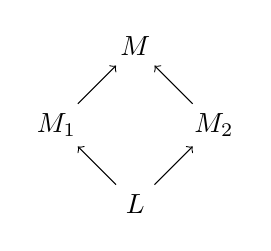
\begin{tikzpicture} %[scale=0.8]
  \node (l) at (0,0) {\(L\)};
  \node (m1) at (-1,1) {\(M_1\)};
  \node (m2) at (1,1) {\(M_2\)};
  \node (m) at (0,2) {\(M\)};
  \draw [->] (l) -- (m1);
  \draw [->] (l) -- (m2);
  \draw [->] (m1) -- (m);
  \draw [->] (m2) -- (m);
\end{tikzpicture}
\]

Let us now formally introduce the refinement of the rules in a poset using the positive influence.

\begin{definition}[Refinement based on positive influence]
  \begin{itemize}
  \item[]
  \item The refinement of two causally consecutive events $\mathcal{R}(e_1< e_2)$ is the sequence:
    \[
    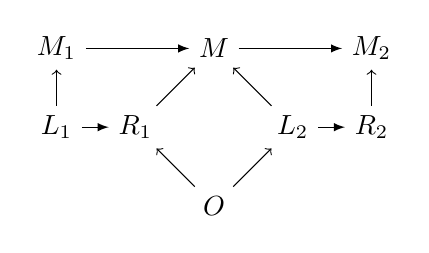
\begin{tikzpicture} %[scale=0.8]
      \node (o) at (0,-1) {\(O\)};
      \node (p) at (0,1) {\(M\)};
      \node (r1) at (-1,0) {\(R_1\)};
      \node (l1) at (-2,0) {\(L_1\)};
      \node (l2) at (1,0) {\(L_2\)};
      \node (r2) at (2,0) {\(R_2\)};
      \node (m1) at (-2,1) {\(M_1\)};
      \node (m2) at (2,1) {\(M_2\)};
      \draw [->] (l1) -- (m1);
      \draw [->] (r2) -- (m2);
      \draw [->] (o) -- (r1);
      \draw [->] (o) -- (l2);
      \draw [->] (r1) -- (p);
      \draw [->] (l2) -- (p);
      \draw [>=latex, ->] (m1) -- (p);
      \draw [>=latex, ->] (p) -- (m2);
      \draw [>=latex, ->] (l1) -- (r1);
      \draw [>=latex, ->] (l2) -- (r2);
    \end{tikzpicture}
    \]
    \item Refinements combine using two combinators:
      \begin{itemize}
      \item the sequence combinator $\mathcal{R}(e_1 < e_2)\oplus\mathcal{R}(e_2 < e_3)$ resulting in the graph in~\autoref{ex:e1e2e3};
      \item the concurrent combinator $\mathcal{R}(e_1 < e)\otimes\mathcal{R}(e_2 < e)$ which combines contexts obtained from $e_1$ and $e_2$ into a single context.
      \end{itemize}
  \item The refinement of a poset $s$ is obtained using the two combinators above and resulting in the sequence
    \[
    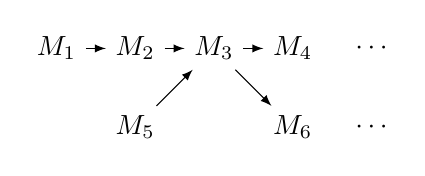
\begin{tikzpicture} %[scale=0.8]
      \node (m1) at (0,0) {\(M_1\)};
      \node (m2) at (1,0) {\(M_2\)};
      \node (m3) at (2,0) {\(M_3\)};
      \node (m4) at (3,0) {\(M_4\)};
      \node (m5) at (1,-1) {\(M_5\)};
      \node (m6) at (3,-1) {\(M_6\)};
      \node (m7) at (4,-1) {\(\cdots\)};
      \node (m8) at (4,0) {\(\cdots\)};
      \draw [>=latex, ->] (m1) -- (m2);
      \draw [>=latex, ->] (m2) -- (m3);
      \draw [>=latex, ->] (m3) -- (m4);
      \draw [>=latex, ->] (m5) -- (m3);
      \draw [>=latex, ->] (m3) -- (m6);
    \end{tikzpicture}
    \]
    where each transition $M_i\action M_j$ denotes a square
    \[
    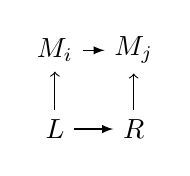
\begin{tikzpicture} %[scale=0.8]
      \node (mi) at (-2,1) {\(M_i\)};
      \node (mj) at (-1,1) {\(M_j\)};
      \node (r1) at (-1,0) {\(R\)};
      \node (l1) at (-2,0) {\(L\)};
      \draw [->] (l1) -- (mi);
      \draw [->] (r1) -- (mj);
      \draw [>=latex, ->] (mi) -- (mj);
      \draw [>=latex, ->] (l1) -- (r1);
    \end{tikzpicture}
    \]
    The refinement of an event in a poset $\mathcal{R}(e\in s)$ is then the square
    \[
    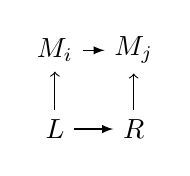
\begin{tikzpicture} %[scale=0.8]
      \node (mi) at (-2,1) {\(M_i\)};
      \node (mj) at (-1,1) {\(M_j\)};
      \node (r1) at (-1,0) {\(R\)};
      \node (l1) at (-2,0) {\(L\)};
      \draw [->] (l1) -- (mi);
      \draw [->] (r1) -- (mj);
      \draw [>=latex, ->] (mi) -- (mj);
      \draw [>=latex, ->] (l1) -- (r1);
    \end{tikzpicture}
    \]
    where $\labl(e) = r$ and $m_{M_i}(e) = L \emb M_i$.
  \end{itemize}
\end{definition}

Let us define the notion of refinement using negative influence.

\begin{definition}[Refinement based on negative influence]
  For two posets $s_1,s_2$ and two events $e_1\in s_1$ and $e_2\in s_2$ let the following be their refinements:
  \begin{align*}
    \mathcal{R}(e_1\in s_1) =
    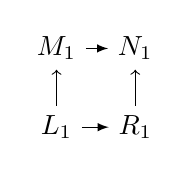
\begin{tikzpicture}[baseline=0.4cm] %[scale=0.8]
      \node (mi) at (-2,1) {\(M_1\)};
      \node (mj) at (-1,1) {\(N_1\)};
      \node (r1) at (-1,0) {\(R_1\)};
      \node (l1) at (-2,0) {\(L_1\)};
      \draw [->] (l1) -- (mi);
      \draw [->] (r1) -- (mj);
      \draw [>=latex, ->] (mi) -- (mj);
      \draw [>=latex, ->] (l1) -- (r1);
    \end{tikzpicture}
    \text{ and }
    \mathcal{R}(e_2\in s_2) =
    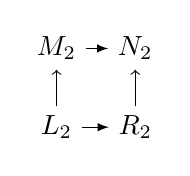
\begin{tikzpicture}[baseline=0.4cm] %[scale=0.8]
      \node (mi) at (-2,1) {\(M_2\)};
      \node (mj) at (-1,1) {\(N_2\)};
      \node (r1) at (-1,0) {\(R_2\)};
      \node (l1) at (-2,0) {\(L_2\)};
      \draw [->] (l1) -- (mi);
      \draw [->] (r1) -- (mj);
      \draw [>=latex, ->] (mi) -- (mj);
      \draw [>=latex, ->] (l1) -- (r1);
    \end{tikzpicture}
  \end{align*}
  Define $\mathcal{R}(e_1\in s_1\redl{-} e_2\in s_2) = M$ for which the diagram below commutes:
  \[
  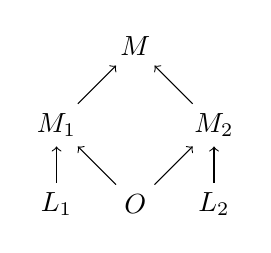
\begin{tikzpicture} %[scale=0.8]
    \node (o) at (0,0) {\(O\)};
    \node (n) at (0,2) {\(M\)};
    \node (l1) at (-1,0) {\(L_1\)};
    \node (l2) at (1,0) {\(L_2\)};
    \node (n1) at (-1,1) {\(M_1\)};
    \node (n2) at (1,1) {\(M_2\)};
    \draw [->] (l1) -- (n1);
    \draw [->] (l2) -- (n2);
    \draw [->] (o) -- (n1);
    \draw [->] (o) -- (n2);
    \draw [->] (n1) -- (n);
    \draw [->] (n2) -- (n);
  \end{tikzpicture}
  \]
\end{definition}

\begin{example}[Feedback loops]

Let us show how we can interpret negative feedback loops. Let $e_1\in s_1\redl{-} e_2\in s_2$ such that $s_2\subset s_1$. Then $e_2\leq_{s_1} e_2$. However this additional constraint does not change the way we interpret negative influence, that is the influence is realised if there exists $M$ such that the following diagram commutes:
\[
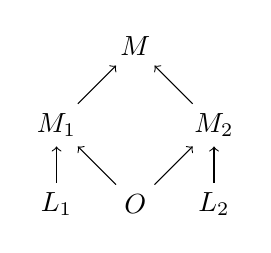
\begin{tikzpicture} %[scale=0.8]
  \node (o) at (0,0) {\(O\)};
  \node (n) at (0,2) {\(M\)};
  \node (l1) at (-1,0) {\(L_1\)};
  \node (l2) at (1,0) {\(L_2\)};
  \node (n1) at (-1,1) {\(M_1\)};
  \node (n2) at (1,1) {\(M_2\)};
  \draw [->] (l1) -- (n1);
  \draw [->] (l2) -- (n2);
  \draw [->] (o) -- (n1);
  \draw [->] (o) -- (n2);
  \draw [->] (n1) -- (n);
  \draw [->] (n2) -- (n);
\end{tikzpicture}
\]
\end{example}

This technique introduces context into the rules. This context might interfere with the intuitive reading of influence.

\begin{example}[Influence on refined rules]
\label{ex:infl_refined}
Let us consider the following two rules:

\begin{verbatim}
r1:  A,B -> A-B
r2:  C,D -> D
\end{verbatim}

Let us additionally consider that rule \verb|r1| occurs in a poset and is refined to \verb|A,B,C -> A-B,C|. We then observe a negative influence of \verb|r2| to \verb|r1|.
\end{example}

If we do not want a negative influence in~\autoref{ex:infl_refined}, we need to refine the definition of influence such that the domain of definition in both rules is considered.

Unrefined rules suggest a local modification on a graph, whereas the refined one are modifications in a larger context. Thus we need to keep in mind the context of the refined rule in order not to overapproximate the influence.

\begin{mdframed}[backgroundcolor=blue!20]
  the definition of influence in refined rules
\end{mdframed}
